\documentclass{ximera}

\graphicspath{{./graphics/}}

\title{Evaluating Limits}
\begin{document}
\begin{abstract}
\end{abstract}
\maketitle

We've seen how we can approach along paths to show that some limits do not exist, but we still don't have any methods for showing that multivariable limits do exist. Our first tool for doing this will be the epsilon-delta definition of a limit, which will allow us to formally prove that a limit exists.

Unfortunately, the epsilon-delta approach has some draw backs. Epsilon-delta proofs can be difficult, and they often require you to either guess or compute the value of a limit prior to starting the proof! So, we will want some easier methods for evaluating limits. One such method will be changing coordinates in a way that reduces our limit to a single variable limit.

\section*{Epsilon-delta definition}

Let's begin by recalling the epsilon-delta definition of a limit from single variable calculus.

\begin{definition}
Let $f:\mathbb{R}\rightarrow\mathbb{R}$ be a function. We write
\[
\lim_{x\rightarrow a} f(x) = L
\]
if for all $\epsilon >0$, there exists some $\delta >0$ such that for all $x$ with $0 < |x-a| < \delta$, we have $|f(x)-L| < \epsilon$.
\end{definition}

We use this definition to guide our formal definition of a limit for multivariable functions.

\begin{definition}
Let $f:\mathbb{R}^n\rightarrow\mathbb{R}$ be a function. We write
\[
\lim_{\vec{x}\rightarrow \vec{a}} f(\vec{x}) = L
\]
if for all $\epsilon >0$, there exists some $\delta >0$ such that for all $\vec{x}$ with $0 < \|\vec{x}-\vec{a}\| < \delta$, we have $|f(\vec{x})-L| < \epsilon$.

We can also state this definition in terms of neighborhoods: $\lim_{\vec{x}\rightarrow \vec{a}} f(\vec{x}) = L$ if, for all $\epsilon>0$, there is some neighborhood of $\vec{a}$ on which $|f(\vec{x})-L| < \epsilon$.
\end{definition}

Because the inputs here are points in $\mathbb{R}^n$, when we take points ``close to'' $\vec{a}$, we do this in terms of distance. Recall that we can compute the distance between points $\vec{x}=(x_1,...,x_n)$ and $\vec{y}=(y_1,...,y_n)$ as
\[
\|\vec{x}-\vec{y}\| = \sqrt{(x_1-y_1)^2+(x_n-y_n)^2}.
\]
So when we're considering all $\vec{x}$ such that $\|\vec{x}-\vec{a}\| < \delta$, we're taking all points within a distance $\delta$ of $\vec{a}$. This is called the \emph{open ball of radius $\delta$ centered at $\vec{a}$}. 

\begin{image}
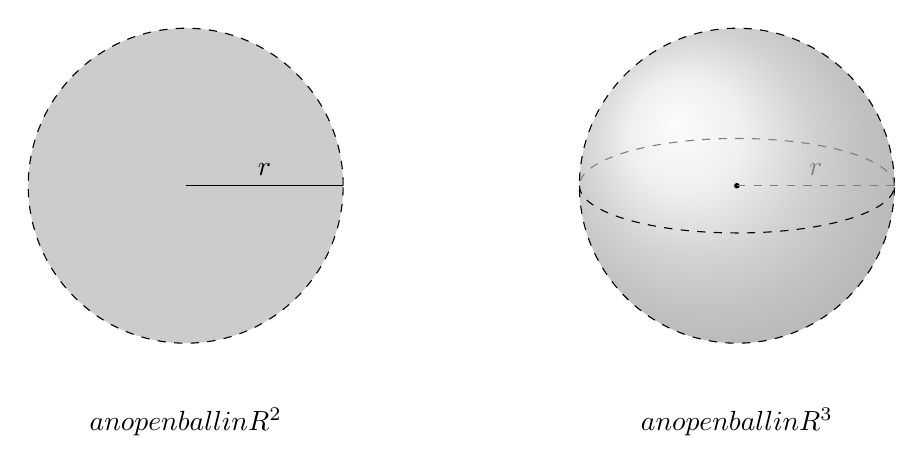
\begin{tikzpicture}
\draw[dashed, fill = gray!40] (0,0) circle (2cm);
\draw (0,0 ) -- node[above]{$r$} (2,0);
\node at (0,-3) {$\text{an open ball in }\mathbb{R}^2$};
\begin{scope}[xshift=7cm]
  \shade[ball color = gray!40, opacity = 0.4] (0,0) circle (2cm);
  \draw[dashed] (0,0) circle (2cm);
  \draw[dashed] (-2,0) arc (180:360:2 and 0.6);
  \draw[dashed, gray] (2,0) arc (0:180:2 and 0.6);
  \fill[fill=black] (0,0) circle (1pt);
  \draw[dashed, gray] (0,0 ) -- node[above]{$r$} (2,0);
  \node at (0,-3) {$\text{an open ball in }\mathbb{R}^3$};
 \end{scope}

\end{tikzpicture}
\end{image}

When we add in the condition that $0<\|\vec{x}-\vec{a}\|$, we are excluding the point $a$ itself.

\begin{example}
We'll prove that $\lim_{\vec{x}\rightarrow (1,2,3)} (2x-y+5z) = 15$, using the epsilon-delta definition of a limit.

Given $\epsilon >0$, we'd like to find $\delta$ such that $0< \|(x,y,z)-(1,2,3)\|<\delta$ guarantees $|(2x-y+5z)-15|<\epsilon$. Let's see what we can get from $0< \|(x,y,z)-(1,2,3)\|<\delta$. We have
\[
0< \sqrt{(x-1)^2+(y-2)^2+(z-3)^2}<\delta.
\]
Using the triangle inequality, $\sqrt{(x-1)^2}+\sqrt{(y-2)^2}+\sqrt{(z-3)^2} < \sqrt{(x-1)^2+(y-2)^2+(z-3)^2}$. From this, we have
\[
0< \sqrt{(x-1)^2}+\sqrt{(y-2)^2}+\sqrt{(z-3)^2}<\delta,
\]
which we can rewrite as
\[
0< |x-1|+|y-2|+|z-3|<\delta.
\]
From this, we have $|x-1|<\delta$, $|y-2|<\delta$, and $|z-3|<\delta$.

Now, let's look at $|(2x-y+5z)-15|$, and try to rewrite this to make use of what we've found so far. We have
\begin{align*}
 |(2x-y+5z)-15| &=|(2x-2)+(-y+2)+(5z-15)|\\
&=|2(x-1)-(y-2)+5(z-3)|\\
&\geq |2(x-1)|+|y-2|+|5(z-3)|,
\end{align*}
using the triangle inequality. By properties of absolute values, and using our above observations, we have
\begin{align*}
|2(x-1)|+|y-2|+|5(z-3)| &= 2|x-1|+|y-2|+5|z-3|\\
&=2\delta + \delta + 5\delta\\
&=8\delta.
\end{align*}
So if we choose $\delta = \epsilon/8$, we'll have $|(2x-y+5z)-15|<\epsilon$ for all $(x,y,z)$ with $0< \|(x,y,z)-(1,2,3)\|<\delta$.
\end{example}

Now that we have a formal definition of limits, let's revisit our result about approaching a point along various paths.

\begin{proposition}
Consider a function $f:\mathbb{R}^n\rightarrow \mathbb{R}$, and a point $\vec{a}\in\mathbb{R}^n$. Suppose there are continuous paths $\vec{x}(t)$ and $\vec{y}(t)$ such that $\vec{x}(t_1) = \vec{y}(t_2) = \vec{a}$, and suppose that
\[
\lim_{t\rightarrow t_1}f(\vec{x}(t))\neq \lim_{t\rightarrow t_2}f(\vec{y}(t))
\]
(or one of these limits does not exist). Then $\lim_{\vec{x}\rightarrow\vec{a}}f(x)$ does not exist.
\end{proposition}

\begin{proof}
In this proof, we'll handle the case where both limits exist. Suppose $\lim_{t\rightarrow t_1}f(\vec{x}(t)) = L$ and $\lim_{t\rightarrow t_2}f(\vec{y}(t)) = M$. We'll prove the contrapositive of the given statement: if $\lim_{\vec{x}\rightarrow\vec{a}}f(x)$ exists, then $L=M$.

Suppose $\lim_{\vec{v}\rightarrow\vec{a}}f(\vec{v})=N$. Then there exists $\delta$ such that for $0< \|\vec{v} - \vec{a}\| < \delta$, we have $|f(\vec{v}) - N| < \epsilon$.

Since $\lim_{t\rightarrow t_1}f(\vec{x}(t)) = L$, there exists some $\delta_1>0$ such that for all $t$ with $0<|t-t_1|<\delta_1$, we have $|f(\vec{x}(t))-L|<\epsilon$. Since $\vec{x}$ is continuous, we can also find some $\delta_1'$ such that $\|\vec{x}(t)-\vec{a}\|<\delta$ for $|t-t_1|<\delta_1'$. Since $\|\vec{x}(t) - \vec{a}\| < \delta$, we also have that $|f(\vec{x}(t)) - N| < \epsilon$. From this, we have that
\begin{align*}
|N-L| &= |N-f(\vec{x}(t)) + f(\vec{x}(t)) - L\\
&\leq |f(\vec{x}(t))-N| + |f(\vec{x}(t)) - L|\\
&< 2\epsilon.
\end{align*}
Since this must be true for all $\epsilon$, we must have $N=L$.

By the same reasoning, applied to the path $\vec{y}$, we have $N=M$. Thus, we would need to have $L=M$.
\end{proof}

\section*{Changing coordinates}

Although doing a delta-epsilon proof can be effective for proving that a limit exists and what it's equal to, we still need to predict the value of a limit before starting such a proof. So, we'd like some other techniques for showing that multivariable limits exist, and for evaluating them.

One strategy for evaluating limits is to change coordinates in a way that reduces our multivariable limit to a single variable limit.

Suppose we're taking the limit of a function $f(x,y)$ as $(x,y)\rightarrow (0,0)$, so we're approaching the origin. In polar coordinates $(\theta, r)$, approaching the origin is equivalent to taking $r\rightarrow 0$. It doesn't matter what $\theta$ does; as long as $r$ goes to $0$, we will be approaching the origin.

\begin{image}
\begin{tikzpicture}
\draw[<->] (-5,0) -- (5,0) node[below] {$x$};
\draw[<->] (0,-5) -- (0,5) node[left] {$y$};
\draw[gray] (0,0) circle (4cm);
\draw[gray] (0,0) circle (2cm);
\draw[gray] (0,0) circle (1cm);
\draw[gray] (0,0) circle (.5cm);
\draw[gray] (0,0) circle (.25cm);
\draw[gray] (0,0) circle (.125cm);
\draw[gray] (0,0) circle (.0625cm);
\node at (3,3) {$r = 1$};
\node at (1.5,1.5) {$r =.5$};
\node at (.75,.75) {$r = .25$};
\node at (0,-5.25) {As $r\rightarrow 0$, we approach the origin.};
\end{tikzpicture}
\end{image}

This makes polar coordinates a common and convenient choice for a change of variables to evaluate limits.

\begin{example}
We'll use polar coordinates to evaluate the limit $\lim_{(x,y)\rightarrow (0,0)}xy$. Changing to polar coordinates, we have
\begin{align*}
\lim_{(x,y)\rightarrow (0,0)}xy &= \lim_{r\rightarrow 0} r\cos\theta \cdot r\sin\theta\\
&= \lim_{r\rightarrow 0} r^2\cos\theta\sin\theta.
\end{align*}
We will use the squeeze theorem to evaluate this limit. Since $-1\leq\cos\theta\sin\theta\leq 1$ for all $\theta$, we have
\[
-r^2\leq r^2\cos\theta\sin\theta\leq r^2.
\]
Since $\lim_{r\rightarrow 0} -r^2 = \lim_{r\rightarrow 0} r^2=0$, by the squeeze theorem, we have
\[
\lim_{r\rightarrow 0} r^2\cos\theta\sin\theta = 0.
\]
Thus, $\lim_{(x,y)\rightarrow (0,0)}xy = 0$.
\end{example}

Similarly, when the domain of a function is $\mathbb{R}^3$, we can use spherical coordinates to evaluate a limit approaching the origin.

\begin{example}
We will use spherical coordinates to evaluate the limit $\lim_{(x,y,z)\rightarrow (0,0,0)}\frac{x^3}{x^2+y^2+z^2}$. Changing to spherical coordinates, we have
\begin{align*}
\lim_{(x,y,z)\rightarrow (0,0,0)}\frac{x^3}{x^2+y^2+z^2} &= \lim_{\rho\rightarrow 0}\frac{(\rho\cos\theta\sin\phi)^3}{(\rho\cos\theta\sin\phi)^2+(\rho\sin\theta\sin\phi)^2+(\rho\cos\phi)^2}\\
&= \lim_{\rho\rightarrow 0}\frac{\rho^3\cos^3\theta\sin^3\phi}{\rho^2\cos^2\theta\sin^2\phi+\rho^2\sin^2\theta\sin^2\phi+\rho^2\cos^2\phi}\\
&= \lim_{\rho\rightarrow 0}\frac{\rho^3\cos^3\theta\sin^3\phi}{(\rho^2\cos^2\theta+\rho^2\sin^2\theta)\sin^2\phi+\rho^2\cos^2\phi}\\
&= \lim_{\rho\rightarrow 0}\frac{\rho^3\cos^3\theta\sin^3\phi}{\rho^2\sin^2\phi+\rho^2\cos^2\phi}\\
&= \lim_{\rho\rightarrow 0}\frac{\rho^3\cos^3\theta\sin^3\phi}{\rho^2}\\
&= \lim_{\rho\rightarrow 0}\rho\cos^3\theta\sin^3\phi.\\
\end{align*}
Since $-1\leq \cos^3\theta\sin^3\phi\leq 1$, we have
\[
-|\rho|\leq \rho\cos^3\theta\sin^3\phi\leq |\rho|.
\]
Since $\lim_{\rho\rightarrow 0}-|\rho| = \lim_{\rho\rightarrow 0}|\rho|=0$, by the squeeze theorem, we have
\[
\lim_{\rho\rightarrow 0}\rho\cos^3\theta\sin^3\phi = 0,
\]
So $\lim_{(x,y,z)\rightarrow (0,0,0)}\frac{x^3}{x^2+y^2+z^2}$.
\end{example}

In other situations, a different change of coordinates might be more useful. For example, linear changes of coordinates might be used.

\begin{example}
We'll use a change of coordinates to evaluate $\lim_{(x,y)\rightarrow(0,0)} (x-y)e^{-(x-y)^2}$. Here, it's convenient to use the linear change of coordinates $y=x-y$ and $v=x+y$. Notice that $(x,y)\rightarrow (0,0)$ is equivalent to $(u,v)\rightarrow (0,0)$. From this, we have
\[
\lim_{(x,y)\rightarrow(0,0)} (x-y)e^{-(x-y)^2} = \lim_{(u,v)\rightarrow (0,0)} ue^{-u^2}.
\]
Notice that the expression on the right depends only on $u$, and not on $v$. Because of this, we can evaluate this limit as
\begin{align*}
\lim_{(u,v)\rightarrow (0,0)} ue^{-u^2} &= \lim_{u\rightarrow 0} ue^{-u^2}\\
&= \lim_{u\rightarrow 0}\frac{u}{e^{u^2}}\\
&= \answer{0}.
\end{align*}
Thus, we have $\lim_{(x,y)\rightarrow(0,0)} (x-y)e^{-(x-y)^2}=0$.

\end{example}

We can also change coordinates to help us show that certain limits do not exist.

\begin{example}
We will use polar coordinates to show that $\lim_{(x,y)\rightarrow (0,0)} \frac{xy}{x^2+y^2}$ doesn't exist. Changing to polar coordinates, we have
\begin{align*}
\lim_{(x,y)\rightarrow (0,0)} \frac{xy}{x^2+y^2} &= \lim_{r\rightarrow 0}\frac{r\cos\theta\cdot r\sin\theta}{r^2}\\
&= \lim_{r\rightarrow 0}\cos\theta \sin\theta.\\
\end{align*}
If we take $\theta = 0$, this is equivalent to approaching the origin along the $x$-axis, and we have $\cos\theta\sin\theta = 0$.

If we take $\theta = \pi/4$, this is equivalent to approaching the origin along the line $y=x$, and we have $\cos\theta\sin\theta = \frac{1}{2}$.

Since we get different values approaching the origin along different paths, we see that $\lim_{(x,y)\rightarrow (0,0)} \frac{xy}{x^2+y^2}$ does not exist.

Note that the change of coordinates here wasn't absolutely necessary. We could have directly evaluated the limits approaching along the $x$-axis and along the line $y=x$, and seen that the limit does not exist. However, sometimes it's easier to see that a limit doesn't exist by attempting a change to polar coordinates, and finding that we end up with a limit that depends on the value of $\theta$.
\end{example}

In all of the above cases, we considered limits approaching the origin. We can use similar techniques to evaluate limits approaching other points, often by translating coordinate systems.

\begin{example}
Consider the limit $\lim_{(x,y)\rightarrow(2,3)} (x-2)(y-3)$. Here, it's convenient to use polar coordinates translated so they're centered at the point $(2,3)$. That is, we let $x = 2+r\cos\theta $ and $y=3+r\sin\theta$, so that $r=0$ when $(x,y)=(2,3)$. Then we can evaluate our limit as
\begin{align*}
\lim_{(x,y)\rightarrow(2,3)} (x-2)(y-3) &= \lim_{r\rightarrow 0}(2+r\cos\theta-2)(3+r\sin\theta -3)\\
&=\lim_{r\rightarrow 0}r\cos\theta\cdot r\sin\theta\\
&= \lim_{r\rightarrow 0}r^2\cos\theta\sin\theta
\end{align*}
Notice that $-r^2\leq r^2\cos\theta\sin\theta\leq r^2$, and $\lim_{r\rightarrow 0}-r^2 = \lim_{r\rightarrow 0}r^2 = 0$. Then, by the squeeze theorem, $\lim_{r\rightarrow 0} r^2\cos\theta\sin\theta =0$. Thus, we have
\[
\lim_{(x,y)\rightarrow(2,3)} (x-2)(y-3) = 0.
\]
\end{example}

\end{document}